\chapter{Diseño técnico}

Hemos definido hasta ahora gran parte de los ingredientes que llevará twinX: quiénes lo van a usar, qué es capaz de hacer, cuánto vamos a tardar en hacerlo y por qué hace falta algo como twinX.

Es hora de ponernos manos a la obra. Pero antes de ello, es necesario aún definir muchas más cosas, todo ello en relación con lo anterior pero a más bajo nivel: cuáles van a ser exactamente nuestras tareas, qué subtareas asociadas tendremos que desarrollar y cómo va a ser la base de datos. Será vez puestos todos los ingredientes a nuestra disposición para cocinarlos cuando podamos comenzar a utilizar nuestras herramientas para conseguir nuestro objetivo.

\section{Listado inicial del producto (product backlog)}

Es cierto que ya sabemos lo que va a ser capaz de hacer twinX en su primera versión, pero no tenemos claros los pequeños pasos a dar para poder completar las grandes tareas que ya conocemos. Por ello, vamos a elaborar un listado de todo lo que tenemos que hacer en orden de preferencia, paso a paso, para poder conseguir nuestros objetivos de manera organizada.

La priorización de la lista de tareas suele estar hecha por el llamado \textit{product owner}; esto es, el propietario del producto final (en este caso, las dos personas mencionadas en la sección ~\ref{eleccionMetodologia}). Sin embargo, en este caso, vamos a obviar la labor de los propietarios, dado que no se está construyendo un producto desde cero, sino que se parte de lo que ya se construyó en TWINS y porque además, la intención de este proyecto no es obtener un producto inmediatamente utilizable, sino como propuesta de donde partir.

Más técnicamente, cada uno de los componentes de esta lista son acciones que el usuario podrá desarrollar. Esto es algo característico de Scrum y su constante enfoque en el usuario, todo ello en relación con su activa participación con el equipo de desarrollo durante todo el proceso. Pues bien, estas capacitaciones que el usuario final tendrá reciben el nombre de \textbf{historias de usuario}, y es la forma que se tiene en esta metodología ágil de nombrar a los clásicos requisitos. Suponen una reducción en la documentación, ya que no se necesitan especificar demasiados elementos a priori. No obstante y como ya comentamos en secciones pasadas, el número de tareas y, por tanto, de historias de usuario, puede variar, pues al comienzo de cada sprint se realiza una reunión para evaluar los trabajos del equipo de desarrollo y se vuelve a revisar la priorización que se ha hecho de las tareas en el \textit{product backlog}.

En referencia a esas «grandes tareas» que hemos mencionado anteriormente y que ya tenemos definidas, podríamos decir que dentro de ellas se esconden otras de menor generalidad que nos son más sencillas de descomponer o comprender a la hora del desarrollo. Es decir, son una serie de historias de usuario encerradas en otra más grande que alberga a todas ellas. Esto se conoce en el argot de Scrum como \textbf{épicas}. Así, «hacer uso del panel de control» sería una épica, pues dentro de ella irían historias de usuario como «ver un listado con todos los tipos de expedientes».

En la tabla \ref{tab:listadoHU} encontramos el backlog genérico del desarrollo, como producto de la síntesis que se puede hacer de las secciones \ref{subsec:propuesta} y~\ref{subsec:sprints}, donde hemos incluido las historias de usuario a desarrollar para la primera versión de twinX, en sus épicas correspondientes. Entendemos que todas las historias numeradas como «x.1», «x.2», ..., «x.n» pertenecen todas a la épica «x». Recordemos también que el significado de «historia de usuario» no es otro que una acción a desarrollar por el usuario final del sistema, por lo que siempre tienen que estar descritas desde su punto de vista. Es asunto del desarrollador el cuestionarse las tareas (de código en su mayoría) que implica realizar cada una de ellas, por lo que para la elaboración del backlog no nos centraremos en esas tareas a llevar a cabo en cuanto a implementación, sino a satisfacción de las necesidades del usuario.

\begin{table}[H]
	\begin{center}
		\begin{adjustbox}{width=1\textwidth}
			\begin{tabular}{ | c | >{\centering\arraybackslash}p{0.75\linewidth} | c | } 
				\hline
					\textbf{Identificador} & \textbf{Descripción} & \textbf{Sprint} \\
				\hline
					\hyperref[tab:HU1]{HU.1} &  Acceso al panel de control. & 1 \\
				\hline
					\hyperref[tab:HU1.1]{HU.1.1} & Listado de usuarios en todo el sistema: consulta, búsqueda, edición y eliminación de registros. & 1 \\
				\hline
					\hyperref[tab:HU1.2]{HU.1.2} & Listado de tipos de expedientes almacenados: consulta, búsqueda, edición y eliminación de registros. & 1 \\
				\hline
					\hyperref[tab:HU1.3]{HU.1.3} & Listado de fases de expedientes almacenadas: consulta, búsqueda, edición y eliminación de registros. & 1 \\
				\hline
					\hyperref[tab:HU1.4]{HU.1.4} & Listado de mails predefinidos almacenados: consulta, búsqueda, edición y eliminación de registros. & 1 \\
				\hline
					\hyperref[tab:HU1.5]{HU.1.5} & Listado de universidades almacenadas: consulta, búsqueda, edición y eliminación de registros. & 1 \\
				\hline
					\hyperref[tab:HU1.6]{HU.1.6} & Listado de países almacenados: consulta, búsqueda, edición y eliminación de registros. & 1 \\
				\hline
					\hyperref[tab:HU2]{HU.2} & Gestionar el trabajo diario de la oficina: estudiantes, expedientes, acuerdos de estudios, convenios y tutores. & 1 \\
				\hline
					\hyperref[tab:HU2.1]{HU.2.1} & Ver la información más importante y de atención prioritaria de un vistazo. & 1 \\
				\hline
					\hyperref[tab:HU2.2]{HU.2.2} & Gestionar los estudiantes: listado y vistas independientes con posibilidad de edición de sus datos. & 1 \\
				\hline
					\hyperref[tab:HU2.3]{HU.2.3} & Gestionar los convenios: listado y vistas independientes con posibilidad de edición de los distintos campos. & 1 \\
				\hline
					\hyperref[tab:HU2.4]{HU.2.4} & Gestionar los expedientes de los estudiantes: listado y vistas independientes con posibilidad de modificar sus fases. & 1 \\
				\hline
					\hyperref[tab:HU2.5]{HU.2.5} & Gestionar los acuerdos de estudios: listado y vistas independientes con posibilidad de consultar los estudiantes relacionados y sus datos. & 1 \\
				\hline
					\hyperref[tab:HU2.6]{HU.2.6} & Ver todos los tutores del sistema y consultar los acuerdos de estudios asociados a los mismos. & 1 \\
				\hline
					\hyperref[tab:HU3]{HU.3} & Planificación de eventos y tareas. & 2 \\
				\hline
					\hyperref[tab:HU3.1]{HU.3.1} & Crear nuevos eventos con tareas asociadas a los mismos. & 2 \\
				\hline
					\hyperref[tab:HU3.2]{HU.3.2} & Configurar avisos de los eventos y tareas que se creen. & 2 \\
				\hline
					\hyperref[tab:HU3.3]{HU.3.3} & Configurar recordatorios personales. & 2 \\
				\hline
					\hyperref[tab:HU4]{HU.4} & Hacer uso de una mensajería entre los usuarios. & 2 \\
				\hline			
			\end{tabular}	
		\end{adjustbox}
		\caption{Listado de historias de usuario}
		\label{tab:listadoHU}
	\end{center}
\end{table}

\section{Historias de usuario}

A continuación, vamos a ofrecer una serie de tarjetas de todas y cada una de estas historias de usuario, planificadas para los dos primeros sprints y priorizadas como se ha especificado en la tabla \ref{tab:listadoHU}.

\begin{table}[H]
	\begin{center}
		\begin{tabular}{ | c | c | c | } 
			\hline
				\textbf{Identificación} & HU1 - Acceso al panel de control & \textbf{Sprint:} 1 \\
			\hline
				\textbf{Descripción} & \multicolumn{2}{>{\centering\arraybackslash}p{0.5\linewidth}|}{El panel de control posibilita al administrador crear, modificar y eliminar la información con la que trabajan los gestores en twinX} \\
			\hline
				\textbf{Pruebas de aceptación} & \multicolumn{2}{>{\centering\arraybackslash}p{0.5\linewidth}|}{
					\begin{itemize}
						\item Se intenta acceder al panel de control desde la sesión de un usuario sin permisos de administrador y el sistema no permite el acceso.
					\end{itemize}
				} \\
			\hline
			\textbf{Tareas} & \multicolumn{2}{>{\centering\arraybackslash}p{0.5\linewidth}|}{
				\begin{itemize}
					\item Crear el módulo de panel de control
					\item Configurar el \textit{layout}
					\item Agregar el módulo a \texttt{config/main.php}
					\item Agregar el nuevo módulo a la cabecera del sitio en el \textit{frontend}
				\end{itemize}
			} \\		
			\hline			
		\end{tabular}	
		\caption{Tabla de la HU1}
		\label{tab:HU1}
	\end{center}
\end{table}



\begin{table}[H]
	\begin{center}
		\begin{tabular}{ | c | c | c | } 
			\hline
			\textbf{Identificación} & \parbox[t]{7cm}{HU1.1 - Listado de usuarios en todo el sistema: consulta, búsqueda, edición y eliminación de registros.}  & \textbf{Sprint:} 1 \\
			\hline
			\textbf{Descripción} & \multicolumn{2}{>{\centering\arraybackslash}p{0.5\linewidth}|}{Un listado para que el administrador pueda ver todos los usuarios del sistema: tutores, estudiantes, gestores y otros posibles administradores. Se podrán editar los permisos y/o datos del usuario en concreto.} \\
			\hline
			\textbf{Pruebas de aceptación} & \multicolumn{2}{>{\centering\arraybackslash}p{0.5\linewidth}|}{
				\begin{itemize}
					\item El usuario a borrar es de tipo  «estudiante» y tiene al menos un acuerdo de estudios registrado en el sistema, por lo que se impide la acción.
					\item Se intenta cambiar el rango de un estudiante a «gestor», pero hay datos relacionados con el estudiante ya guardados (acuerdo de estudios, expedientes...), por lo que se impide la acción.
					\item Se crea un usuario nuevo, pero se avisa al administrador que dicho usuario aún tiene que activar su cuenta.
				\end{itemize}
			} \\
			\hline
			\textbf{Tareas} & \multicolumn{2}{>{\centering\arraybackslash}p{0.5\linewidth}|}{
				\begin{itemize}
					\item Construir el modelo de Usuario con Gii.
					\item Construir la tabla CRUD\footnotemark con Gii.
				\end{itemize}
			} \\		
			\hline			
		\end{tabular}	
		\caption{Tabla de la HU1.1}
		\label{tab:HU1.1}
	\end{center}
\end{table}~
\footnotetext{Create, Read, Update \& Delete (crear, leer, actualizar y borrar)}


\begin{table}[H]
	\begin{center}
		\begin{tabular}{ | c | c | c | } 
			\hline
			\textbf{Identificación} & \parbox[t]{7cm}{HU1.2 - Listado de tipos de expedientes almacenados: consulta, búsqueda, edición y eliminación de registros.}  & \textbf{Sprint:} 1 \\
			\hline
			\textbf{Descripción} & \multicolumn{2}{>{\centering\arraybackslash}p{0.5\linewidth}|}{El administrador podrá crear, modificar, buscar y eliminar tipos de expedientes para que los gestores puedan especificar nuevos estados en la movilidad de un estudiante concreto.} \\
			\hline
			\textbf{Pruebas de aceptación} & \multicolumn{2}{>{\centering\arraybackslash}p{0.5\linewidth}|}{
				\begin{itemize}
					\item Se intenta borrar un tipo de expediente que está en uso y se deniega la acción.
					\item Se modifica el nombre de un expediente en uso y se alerta al administrador de ello. La acción se realiza después de una confirmación.
				\end{itemize}
			} \\
			\hline
			\textbf{Tareas} & \multicolumn{2}{>{\centering\arraybackslash}p{0.5\linewidth}|}{
				\begin{itemize}
					\item Construir el modelo de tipo de expediente con Gii.
					\item Construir la tabla CRUD con Gii.
				\end{itemize}
			} \\		
			\hline			
		\end{tabular}	
		\caption{Tabla de la HU1.2}
		\label{tab:HU1.2}
	\end{center}
\end{table}

\begin{table}[H]
	\begin{center}
		\begin{tabular}{ | c | c | c | } 
			\hline
			\textbf{Identificación} & \parbox[t]{7cm}{HU1.3 - Listado de fases de expedientes almacenadas: consulta, búsqueda, edición y eliminación de registros.}  & \textbf{Sprint:} 1 \\
			\hline
			\textbf{Descripción} & \multicolumn{2}{>{\centering\arraybackslash}p{0.5\linewidth}|}{El administrador podrá crear, modificar, buscar y eliminar fases de expedientes para poder especificar los eventos que suceden durante la tramitación de un expediente para un estudiante en concreto.} \\
			\hline
			\textbf{Pruebas de aceptación} & \multicolumn{2}{>{\centering\arraybackslash}p{0.5\linewidth}|}{
				\begin{itemize}
					\item Se intenta borrar una fase de expediente que está en uso y se deniega la acción.
					\item Se modifica el nombre de una fase de expediente en uso y se alerta al administrador de ello. La acción se realiza después de una confirmación.
				\end{itemize}
			} \\
			\hline
			\textbf{Tareas} & \multicolumn{2}{>{\centering\arraybackslash}p{0.5\linewidth}|}{
				\begin{itemize}
					\item Construir el modelo de fase de expediente con Gii.
					\item Construir la tabla CRUD con Gii.
					\item Enlazar los nombres de los tipos de expedientes haciendo una consulta a la tabla correspondiente.
					\item Adjuntar una vista para enlazar envíos de mails por defecto al procesar la fase.
				\end{itemize}
			} \\		
			\hline			
		\end{tabular}	
		\caption{Tabla de la HU1.3}
		\label{tab:HU1.3}
	\end{center}
\end{table}

\begin{table}[H]
	\begin{center}
		\begin{tabular}{ | c | c | c | } 
			\hline
			\textbf{Identificación} & \parbox[t]{7cm}{HU1.4 - Listado de mails predefinidos almacenados: consulta, búsqueda, edición y eliminación de registros.\smallskip}  & \textbf{Sprint:} 1 \\
			\hline
			\textbf{Descripción} & \multicolumn{2}{>{\centering\arraybackslash}p{0.5\linewidth}|}{El administrador podrá crear, modificar, buscar y eliminar mails predefinidos que poder adjuntar a una o varias fases en concreto para que sean enviados de forma automatizada al procesar la fase en cuestión.} \\
			\hline
			\textbf{Pruebas de aceptación} & \multicolumn{2}{>{\centering\arraybackslash}p{0.5\linewidth}|}{
				\begin{itemize}
					\item Se intenta eliminar un mail predefinido que está en uso en alguna fase y se deniega la acción
				\end{itemize}
			} \\
			\hline
			\textbf{Tareas} & \multicolumn{2}{>{\centering\arraybackslash}p{0.5\linewidth}|}{
				\begin{itemize}
					\item Construir el modelo con Gii.
					\item Contruir la tabla CRUD con Gii.
					\item Modificar los atributos a mostrar para que se muestren los nombres y no las claves primarias en base de datos.
				\end{itemize}
			} \\		
			\hline			
		\end{tabular}	
		\caption{Tabla de la HU1.4}
		\label{tab:HU1.4}
	\end{center}
\end{table}

\begin{table}[H]
	\begin{center}
		\begin{tabular}{ | c | c | c | } 
			\hline
			\textbf{Identificación} & \parbox[t]{7cm}{HU1.5 - Listado de universidades almacenadas: consulta, búsqueda, edición y eliminación de registros.}  & \textbf{Sprint:} 1 \\
			\hline
			\textbf{Descripción} & \multicolumn{2}{>{\centering\arraybackslash}p{0.5\linewidth}|}{El administrador podrá crear, modificar, buscar y eliminar universidades para que puedan ser elegidas a la hora de especificar los datos de un convenio dado.} \\
			\hline
			\textbf{Pruebas de aceptación} & \multicolumn{2}{>{\centering\arraybackslash}p{0.5\linewidth}|}{
				\begin{itemize}
					\item Se intenta eliminar una universidad en uso y se impide la acción.
					\item Se intenta modificar una universidad en uso y se alerta al usuario de los riesgos. La acción se realiza tras una confirmación.
				\end{itemize}
			} \\
			\hline
			\textbf{Tareas} & \multicolumn{2}{>{\centering\arraybackslash}p{0.5\linewidth}|}{
				\begin{itemize}
					\item Construir el modelo de universidad con Gii.
					\item Construir la tabla CRUD con Gii.
				\end{itemize}
			} \\		
			\hline			
		\end{tabular}	
		\caption{Tabla de la HU1.5}
		\label{tab:HU1.5}
	\end{center}
\end{table}

\begin{table}[H]
	\begin{center}
		\begin{tabular}{ | c | c | c | } 
			\hline
			\textbf{Identificación} & \parbox[t]{7cm}{HU1.6 - Listado de países almacenados: consulta, búsqueda, edición y eliminación de registros.}  & \textbf{Sprint:} 1 \\
			\hline
			\textbf{Descripción} & \multicolumn{2}{>{\centering\arraybackslash}p{0.5\linewidth}|}{El administrador podrá crear, modificar, buscar y eliminar países para su asociación con universidades, todo ello en relación con la creación de convenios.} \\
			\hline
			\textbf{Pruebas de aceptación} & \multicolumn{2}{>{\centering\arraybackslash}p{0.5\linewidth}|}{
				\begin{itemize}
					\item Se intenta eliminar un país en uso y se impide la acción.
					\item Se intenta modificar un país en uso y se alerta al usuario de los riesgos. La acción se realiza tras una confirmación.
				\end{itemize}
			} \\
			\hline
			\textbf{Tareas} & \multicolumn{2}{>{\centering\arraybackslash}p{0.5\linewidth}|}{
				\begin{itemize}
					\item Construir el modelo de país con Gii.
					\item Construir la tabla CRUD con Gii.
				\end{itemize}
			} \\		
			\hline			
		\end{tabular}	
		\caption{Tabla de la HU1.6}
		\label{tab:HU1.6}
	\end{center}
\end{table}

\begin{table}[H]
	\begin{center}
		\begin{tabular}{ | c | c | c | } 
			\hline
			\textbf{Identificación} & \parbox[t]{7cm}{HU2 - Gestionar el trabajo diario de la oficina: estudiantes, expedientes, acuerdos de estudios, convenios y tutores.\smallskip}  & \textbf{Sprint:} 1 \\
			\hline
			\textbf{Descripción} & \multicolumn{2}{>{\centering\arraybackslash}p{0.5\linewidth}|}{El menú de gestión es el que frecuentarán los trabajadores de la oficina, donde gestionarán todo lo que rodea a la movilidad internacional en la facultad.} \\
			\hline
			\textbf{Pruebas de aceptación} & \multicolumn{2}{>{\centering\arraybackslash}p{0.5\linewidth}|}{
				\begin{itemize}
					\item Se intenta acceder a gestión desde la sesión de un usuario sin permisos de gestor y el sistema no permite el acceso.
				\end{itemize}
			} \\
			\hline
			\textbf{Tareas} & \multicolumn{2}{>{\centering\arraybackslash}p{0.5\linewidth}|}{
				\begin{itemize}
					\item Crear el módulo de gestión
					\item Configurar el \textit{layout}
					\item Agregar el módulo a \texttt{config/main.php}
					\item Agregar el nuevo módulo a la cabecera del sitio en el \textit{frontend}
				\end{itemize}
			} \\		
			\hline				
		\end{tabular}	
		\caption{Tabla de la HU2}
		\label{tab:HU2}
	\end{center}
\end{table}

\begin{table}[H]
	\begin{center}
		\begin{tabular}{ | c | c | c | } 
			\hline
			\textbf{Identificación} & \parbox[t]{7cm}{HU2.1 - Ver la información más importante y de atención prioritaria de un vistazo.\smallskip}  & \textbf{Sprint:} 1 \\
			\hline
			\textbf{Descripción} & \multicolumn{2}{>{\centering\arraybackslash}p{0.5\linewidth}|}{Disposición de un panel que resuma todo lo más importante que un gestor deba atender en un día concreto; esto es, que resuma los asuntos a atender en una sola visa. Esta utilidad recibe el nombre de \textit{dashboard}} \\
			\hline
			\textbf{Pruebas de aceptación} & \multicolumn{2}{>{\centering\arraybackslash}p{0.5\linewidth}|}{
				\begin{itemize}
					\item Si una tarjeta tiene mucho contenido, solo se mostrará una parte del mismo, para no entorpecer la visibilidad de las demás tarjetas.
					\item Si una tarjeta no tiene contenido, se tendrá que avisar de ello en lugar de dejarla en blanco.
				\end{itemize}
			} \\
			\hline
			\textbf{Tareas} & \multicolumn{2}{>{\centering\arraybackslash}p{0.5\linewidth}|}{
				\begin{itemize}
					\item Crear la interfaz gráfica siguiendo los bocetos.
					\item Asociar cada tarjeta de información con los registros necesarios en la base de datos.
				\end{itemize}
			} \\		
			\hline			
		\end{tabular}	
		\caption{Tabla de la HU2.1}
		\label{tab:HU2.1}
	\end{center}
\end{table}

\begin{table}[H]
	\begin{center}
		\begin{tabular}{ | c | c | c | } 
			\hline
			\textbf{Identificación} & \parbox[t]{7cm}{HU2.2 - Gestionar los estudiantes: listado y vistas independientes con posibilidad de edición de los distintos campos.}  & \textbf{Sprint:} 1 \\
			\hline
			\textbf{Descripción} & \multicolumn{2}{>{\centering\arraybackslash}p{0.5\linewidth}|}{Los gestores dispondrán de una lista con todos los estudiantes con algún proceso de movilidad registrado. Desde ahí, podrán acceder a otros menús en relación con un estudiante en concreto.} \\
			\hline
			\textbf{Pruebas de aceptación} & \multicolumn{2}{>{\centering\arraybackslash}p{0.5\linewidth}|}{
				\begin{itemize}
					\item Se intenta acceder al acuerdo de estudios de un estudiante que no tiene. Se muestra un mensaje de error.
				\end{itemize}
			} \\
			\hline
			\textbf{Tareas} & \multicolumn{2}{>{\centering\arraybackslash}p{0.5\linewidth}|}{
				\begin{itemize}
					\item Construir el modelo de estudiante con Gii.
					\item Costruir la tabla CRUD con Gii.
					\item Desarrollar la vista de un estudiante.
					\item Programar acciones especiales para cada entrada en la lista (acceso a acuerdo de estudios, convenio, expedientes...)
				\end{itemize}
			} \\		
			\hline			
		\end{tabular}	
		\caption{Tabla de la HU2.2}
		\label{tab:HU2.2}
	\end{center}
\end{table}

\begin{table}[H]
	\begin{center}
		\begin{tabular}{ | c | c | c | } 
			\hline
			\textbf{Identificación} & \parbox[t]{7cm}{HU2.3 - Gestionar los convenios: listado y vistas independientes con posibilidad de edición de los distintos campos.}  & \textbf{Sprint:} 1 \\
			\hline
			\textbf{Descripción} & \multicolumn{2}{>{\centering\arraybackslash}p{0.5\linewidth}|}{Los gestores dispondrán de una lista con todos los convenios registrados en el sistema. Podrán consultarlos, buscarlos, añadir nuevos, editarlos y borrarlos. También podrán ver los estudiantes asociados a un convenio concreto para los que se tiene un acuerdo de estudios vigente.
			} \\
			\hline
			\textbf{Pruebas de aceptación} & \multicolumn{2}{>{\centering\arraybackslash}p{0.5\linewidth}|}{
				\begin{itemize}
					\item Se intenta eliminar un convenio que tiene algún acuerdo de estudios vigente. No se lleva a cabo la acción y se alerta al usuario.
				\end{itemize}
			} \\
			\hline
			\textbf{Tareas} & \multicolumn{2}{>{\centering\arraybackslash}p{0.5\linewidth}|}{
				\begin{itemize}
					\item Crear el modelo de convenio con Gii.
					\item Crear la tabla CRUD con Gii.
					\item Crear la interfaz para la vista de convenios acorde con los bocetos y las necesidades.
				\end{itemize}
			} \\		
			\hline			
		\end{tabular}	
		\caption{Tabla de la HU2.3}
		\label{tab:HU2.3}
	\end{center}
\end{table}

\begin{table}[H]
	\begin{center}
		\begin{tabular}{ | c | c | c | } 
			\hline
			\textbf{Identificación} & \parbox[t]{7cm}{HU2.4 - Gestionar los expedientes: listado y vistas independientes con posibilidad de edición de los distintos campos.}  & \textbf{Sprint:} 1 \\
			\hline
			\textbf{Descripción} & \multicolumn{2}{>{\centering\arraybackslash}p{0.5\linewidth}|}{Los gestores dispondrán de una lista con todos los expedientes registrados en el sistema. Podrán consultarlos, buscarlos, añadir nuevos, editarlos y borrarlos. Dispondrán de un menú interno al que acceder para ver los historiales de los expedientes: las fases por las que han pasado, ejecutar algún cambio de fase o consultar datos relacionados con los estudiantes, sus acuerdos y los convenios asociados.
			} \\
			\hline
			\textbf{Pruebas de aceptación} & \multicolumn{2}{>{\centering\arraybackslash}p{0.5\linewidth}|}{
				\begin{itemize}
					\item Se intenta procesar más de una fase al mismo tiempo. No se lleva a cabo la acción y se alerta al usuario.
				\end{itemize}
			} \\
			\hline
			\textbf{Tareas} & \multicolumn{2}{>{\centering\arraybackslash}p{0.5\linewidth}|}{
				\begin{itemize}
					\item Crear el modelo de expediente con Gii.
					\item Crear la tabla CRUD con Gii.
					\item Diseñar la interfaz gráfica de acuerdo con los bocetos y las necesidades.
					\item Crear los accesos directos a la vista de estudiante y a la de convenio.
				\end{itemize}
			} \\		
			\hline			
		\end{tabular}	
		\caption{Tabla de la HU2.4}
		\label{tab:HU2.4}
	\end{center}
\end{table}

\begin{table}[H]
	\begin{center}
		\begin{tabular}{ | c | c | c | } 
			\hline
			\textbf{Identificación} & \parbox[t]{7cm}{HU2.5 - Gestionar los acuerdos de estudios: listado y vistas independientes con posibilidad de edición de los distintos campos.}  & \textbf{Sprint:} 1 \\
			\hline
			\textbf{Descripción} & \multicolumn{2}{>{\centering\arraybackslash}p{0.5\linewidth}|}{Los gestores dispondrán de una lista con todos los acuerdos de estudios registrados en el sistema. Podrán consultarlos, buscarlos, añadir nuevos, editarlos y borrarlos. También podrán ver el convenio al que se asocia un acuerdo de estudios dado y los expedientes de ese acuerdo para con el estudiante que lo tiene registrado.
			} \\
			\hline
			\textbf{Pruebas de aceptación} & \multicolumn{2}{>{\centering\arraybackslash}p{0.5\linewidth}|}{
				\begin{itemize}
					\item Se intenta eliminar un acuerdo vigente. No se lleva a cabo la acción y se alerta al usuario.
				\end{itemize}
			} \\
			\hline
			\textbf{Tareas} & \multicolumn{2}{>{\centering\arraybackslash}p{0.5\linewidth}|}{
				\begin{itemize}
					\item Crear el modelo de convenio con Gii.
					\item Crear la tabla CRUD con Gii.
					\item Crear los accesos directos a la vista de estudiante y a la de convenio.
				\end{itemize}
			} \\		
			\hline			
		\end{tabular}	
		\caption{Tabla de la HU2.5}
		\label{tab:HU2.5}
	\end{center}
\end{table}

\begin{table}[H]
	\begin{center}
		\begin{tabular}{ | c | c | c | } 
			\hline
			\textbf{Identificación} & \parbox[t]{7cm}{HU2.6 - Ver todos los tutores del sistema y consultar los acuerdos de estudios asociados a los mismos.\smallskip}  & \textbf{Sprint:} 1 \\
			\hline
			\textbf{Descripción} & \multicolumn{2}{>{\centering\arraybackslash}p{0.5\linewidth}|}{Los gestores dispondrán de una lista con todos los tutores activos en el sistema (esto es, tutorizando algún acuerdo de estudios). Podrán consultarlos, buscarlos y ver información relacionada, como los acuerdos de estudios que tutoriza. También se podrá asignar un tutor a un acuerdo de estudios existente y que no tenga tutor previamente.
			} \\
			\hline
			\textbf{Pruebas de aceptación} & \multicolumn{2}{>{\centering\arraybackslash}p{0.5\linewidth}|}{
				\begin{itemize}
					\item Se intenta asignar un tutor a un acuerdo de estudios que ya tiene tutor o el cual no se encuentra vigente. No se lleva a cabo la acción y se alerta al usuario.
				\end{itemize}
			} \\
			\hline
			\textbf{Tareas} & \multicolumn{2}{>{\centering\arraybackslash}p{0.5\linewidth}|}{
				\begin{itemize}
					\item Crear el modelo de tutor con Gii.
					\item Crear la tabla CRUD con Gii.
					\item Crear los accesos directos a la vista de acuerdo de estudios.
				\end{itemize}
			} \\		
			\hline			
		\end{tabular}	
		\caption{Tabla de la HU2.6}
		\label{tab:HU2.6}
	\end{center}
\end{table}

\begin{table}[H]
	\begin{center}
		\begin{tabular}{ | c | c | c | } 
			\hline
			\textbf{Identificación} & \parbox[t]{7cm}{HU3 - Planificación de eventos y tareas.}  & \textbf{Sprint:} 2 \\
			\hline
			\textbf{Descripción} & \multicolumn{2}{>{\centering\arraybackslash}p{0.5\linewidth}|}{Los gestores tendrán la posibilidad de crear eventos y tareas para organizar mejor su trabajo} \\
			\hline
			\textbf{Pruebas de aceptación} & \multicolumn{2}{>{\centering\arraybackslash}p{0.5\linewidth}|}{
				\begin{itemize}
					\item Se intenta visualizar el calendario sin permisos mínimos de gestor. La plataforma deniega el acceso.
				\end{itemize}
			} \\
			\hline
			\textbf{Tareas} & \multicolumn{2}{>{\centering\arraybackslash}p{0.5\linewidth}|}{
				\begin{itemize}
					\item Crear el módulo de calendario.
					\item Configurar el \textit{layout}.
					\item Agregar el módulo a \texttt{config/main.php}.
					\item Agregar el nuevo módulo a la cabecera del sitio en el \textit{frontend}.
				\end{itemize}
			} \\		
			\hline			
		\end{tabular}	
		\caption{Tabla de la HU3}
		\label{tab:HU3}
	\end{center}
\end{table}

\begin{table}[H]
	\begin{center}
		\begin{tabular}{ | c | c | c | } 
			\hline
			\textbf{Identificación} & \parbox[t]{7cm}{HU3.1 - Crear nuevos eventos con tareas asociadas a los mismos.\smallskip}  & \textbf{Sprint:} 2 \\
			\hline
			\textbf{Descripción} & \multicolumn{2}{>{\centering\arraybackslash}p{0.5\linewidth}|}{Los gestores podrán crear eventos comunes a todo el personal de gestión de la plataforma y complementarlos usando tareas.} \\
			\hline
			\textbf{Pruebas de aceptación} & \multicolumn{2}{>{\centering\arraybackslash}p{0.5\linewidth}|}{
				\begin{itemize}
					\item Se intenta crear un evento con una fecha anterior a la actual y el sistema alerta del error e impide la operación.
					\item Se intenta eliminar un evento que no ha finalizado y que tiene tareas pendientes. El sistema avisa y efectúa la acción tras una confirmación.
				\end{itemize}
			} \\
			\hline
			\textbf{Tareas} & \multicolumn{2}{>{\centering\arraybackslash}p{0.5\linewidth}|}{
				\begin{itemize}
					\item Crear los modelos de evento y tarea con Gii.
					\item Crear la tabla CRUD con Gii y modificarla de acuerdo con los bocetos.
					\item Diseñar la interfaz de usuario para la creación de eventos y tareas.
				\end{itemize}
			} \\		
			\hline			
		\end{tabular}	
		\caption{Tabla de la HU3.1}
		\label{tab:HU3.1}
	\end{center}
\end{table}

\begin{table}[H]
	\begin{center}
		\begin{tabular}{ | c | c | c | } 
			\hline
			\textbf{Identificación} & \parbox[t]{7cm}{HU3.2 - Configurar avisos de los eventos y tareas que se creen.}  & \textbf{Sprint:} 2 \\
			\hline
			\textbf{Descripción} & \multicolumn{2}{>{\centering\arraybackslash}p{0.5\linewidth}|}{Los gestores podrán asignar avisos a los eventos y tareas creados para ser notificados cuando elijan y a la persona a la que se los asignen.} \\
			\hline
			\textbf{Pruebas de aceptación} & \multicolumn{2}{>{\centering\arraybackslash}p{0.5\linewidth}|}{
				\begin{itemize}
					\item Se intenta poner un recordatorio en una fecha anterior a la actual. El sistema lo notifica e impide la acción.
				\end{itemize}
			} \\
			\hline
			\textbf{Tareas} & \multicolumn{2}{>{\centering\arraybackslash}p{0.5\linewidth}|}{
				\begin{itemize}
					\item Construir el modelo de la tabla \texttt{deadline\_aviso} con Gii.
					\item Modificar las vistas de calendario y tarea para agregar los recordatorios.
					\item Añadir al menú de notificaciones la aparición de avisos por evento o tarea pendiente.
				\end{itemize}
			} \\		
			\hline			
		\end{tabular}	
		\caption{Tabla de la HU3.2}
		\label{tab:HU3.2}
	\end{center}
\end{table}

\begin{table}[H]
	\begin{center}
		\begin{tabular}{ | c | c | c | } 
			\hline
			\textbf{Identificación} & \parbox[t]{7cm}{HU3.3 - Configurar los recordatorios personales.}  & \textbf{Sprint:} 2 \\
			\hline
			\textbf{Descripción} & \multicolumn{2}{>{\centering\arraybackslash}p{0.5\linewidth}|}{Los gestores tendrán la posibilidad de programar recordatorios para recibir un aviso en el futuro.} \\
			\hline
			\textbf{Pruebas de aceptación} & \multicolumn{2}{>{\centering\arraybackslash}p{0.5\linewidth}|}{
				\begin{itemize}
					\item Se intenta programar un recordatorio para una fecha anterior a la actual. El sistema lanza una aviso e impide la acción.
				\end{itemize}
			} \\
			\hline
			\textbf{Tareas} & \multicolumn{2}{>{\centering\arraybackslash}p{0.5\linewidth}|}{
				\begin{itemize}
					\item Construir el modelo de recordatorio con Gii.
					\item Construir la tabla CRUD con Gii.
					\item Configurar el panel de notificaciones para que muestre también los recordatorios programados.
				\end{itemize}
			} \\		
			\hline			
		\end{tabular}	
		\caption{Tabla de la HU3.3}
		\label{tab:HU3.3}
	\end{center}
\end{table}

\begin{table}[H]
	\begin{center}
		\begin{tabular}{ | c | c | c | } 
			\hline
			\textbf{Identificación} & \parbox[t]{7cm}{HU4 - Hacer uso de la mensajería entre los usuarios.\smallskip}  & \textbf{Sprint:} 2 \\
			\hline
			\textbf{Descripción} & \multicolumn{2}{>{\centering\arraybackslash}p{0.5\linewidth}|}{Los usuarios pueden enviarse mensajes entre ellos mismos: consultar los mensajes recibidos, escribir nuevos y cambiar la etiqueta de los ya existentes (importante, eliminado, etc.)} \\
			\hline
			\textbf{Pruebas de aceptación} & \multicolumn{2}{>{\centering\arraybackslash}p{0.5\linewidth}|}{
				\begin{itemize}
					\item Se intenta enviar un mensaje a un usuario no existente. El sistema alerta del error y el mensaje no es enviado.
				\end{itemize}
			} \\
			\hline
			\textbf{Tareas} & \multicolumn{2}{>{\centering\arraybackslash}p{0.5\linewidth}|}{
				\begin{itemize}
					\item Construir el modelo de mensaje con Gii.
					\item Construir la tabla CRUD con Gii.
					\item Modificar la interfaz para asemejarla a una bandeja de entrada de mensajes.
					\item Configurar las notificaciones de recepción de mensajes.
				\end{itemize}
			} \\		
			\hline			
		\end{tabular}	
		\caption{Tabla de la HU4}
		\label{tab:HU4}
	\end{center}
\end{table}

Hemos plasmado un total de 19 historias de usuario, con las tareas que implicará cada una. Es obvio que en la práctica, no solo variará el número de tareas asociado a las HHUU, sino que muy probablemente, tampoco acabemos implementando exactamente las que tenemos aquí, sino que podrían surgir otras o incluso cambiar la priorización de unas a otras en el cambio del sprint 1 al 2. Sobre la implementación de las historias de usuario y el progreso que las acompaña, hablaremos en el capítulo \ref{implementacion}

\section{Modelo de la base de datos}
\label{sec:modelobd}

Cada vez tenemos una idea más clara de cómo va a ser twinX, pero antes hemos de especificar uno de los puntos más importantes para hacer posible el producto final como es la base de datos. En ella, tenemos que especificar las restricciones que hay, cuáles atributos tienen que ser compartidos entre tablas (claves externas), cuáles no se pueden repetir en una relación (claves primarias) y cuáles no pueden estar vacíos.

Nótese la importancia de dedicar tiempo al desarrollo de esta tarea: estableciendo las restricciones necesarias, aunque tengamos algún olvido a la hora de implementar la interfaz con la que el usuario interaccionará, siempre tendremos el respaldo de que la base de datos no comprometerá su estado de consistencia. Por ejemplo, no podemos dejar que se elimine un acuerdo de estudios para el cual hay algún estudiante registrado. O incluso tampoco podemos crear más de un acuerdo de estudios para un estudiante por curso.

El modelo de la base de datos creado es el que se propone en la figura \ref{fig:modeloBD}. El análisis ha dado lugar a un total de 30 tablas, donde se contemplan funcionalidades que no están previstas de implementación en los dos primeros sprints, como son por ejemplo el historial de mensajes enviados, los acuerdos favoritos de un gestor o la confección del acuerdo de estudios a través de la plataforma. No obstante, el diseño se ha pensado para tener en cuenta el futuro desarrollo de twinX y así no desviarlo de la línea de las ideas principales que ya hay definidas. El diagrama ha sido realizado con la herramienta dbdiagram.io \cite{dbdiagram}.

\begin{figure}[H]
	\centering
	\includegraphics[page=2,width=\textwidth,height=\textheight,trim=0 0 0 10cm, clip=true]{pdf/modelo_bd}
	\label{fig:modeloBD}
	\caption{Modelo de la base de datos de twinX}
\end{figure}

El cambio con respecto a TWINS es muy grande. Si bien es cierto que en la aplicación ya existente se pueden encontrar tablas para fines varios que no figuran en la planificación de twinX, hay muchas tablas que pueden evitarse; aunque, sobre todo, prima la duplicidad y redundancia de atributos. Por ejemplo, en TWINS se almacenaban algunos atributos como la nota extra que se tiene al optar por una plaza de movilidad en función de las competencias lingüísticas, algo que es fácilmente calculable comparando los requisitos que exige el convenio y las competencias del estudiante. En función de ello, se puede asignar una mayor nota si procede.

Del modelo, destaca la extensión de la tablad de convenios, donde hay mucha información que guardar. Hay campos para los que ha sido complicado escoger un nombre para definir el atributo; más concretamente, estos pueden ser los de comienzo y fin de las nominaciones, apliaciones y los de la movilidad (begin\_nom\_1s correspondería a «fecha de comienzo de la movilidad en el primer semestre», etc.). Uno de los puntos clave estará en disponer toda esta información de manera organizada, para ofrecer al usuario una buena experiencia pero aportando, al mismo tiempo, facilidad de uso y practicidad para con su trabajo diario.

Otra tabla importante, aunque no extensa, es la de usuario. Tiene muchas relaciones, ya que puede ser definida como una especificación con tutor, gestor, administrador, y estudiante. Ya que en futuras versiones twinX pretende ofrecer acceso a los estudiantes también para sus gestiones, se ha incluido en esta tabla los atributos comunes a todo el público del portal. Como consecuencia, esto nos ahorra tener una tabla con gestores o tutores, pues tan solo habría que especificar esto con un atributo (\texttt{tipo\_usuario}), algo que en TWINS estaba separado, aumentando el número de tablas. Esto también es aplicable a la tabla \texttt{deadline\_aviso}, donde se aglomeran los avisos tanto ligados a eventos en general como a las tareas creadas para un evento.

Por último, comentaremos que para el envío de mensajes predefinidos de forma automatizada al cambiar un \gls{ExpedientetwinX} de \gls{FaseExpedientetwinX} tiene un registro a modo de historial en la tabla \texttt{hist\_envio\_mail\_fase} y que se establece una alternativa (\texttt{hist\_envio\_mail\_fase\_mod}) para cuando se quiera enviar un email que no está predefinido, conducta que ya se aprecia en TWINS, donde se guarda el texto completo de cada correo que se manda, esté o no predefinido en la base de datos.

\section{Arquitectura de twinX}

Para el desarrollo de twinX vamos a emplear, como era de esperar una vez sabido que se trata de un sistema web, la patrón arquitectónico Modelo-Vista-Controlador (MVC). Enfocado en la modularización, separamos estas tres entidades para poder dejar de un lado los datos (\textbf{modelo}), que complementan a la interfaz gráfica (\textbf{vista}), todo ello impulsado y organizado por el \textbf{controlador}, que actúa de mediador entre ambas entidades.

Este aislamiento de unidades funcionales facilita la comprensión y hace que sea mucho más sencillo modificar una unidad particular de todo el sistema, sin necesidad de conocer el funcionamiento de las demás. Pensemos que en proyectos de mayor envergadura, esto es muy potente, puesto que una persona podría dedicarse al mantenimiento de una única parte de todo el conjunto, lo que dotaría al desarrollador de independencia para poder realizar su trabajo de forma individual sin tener que recurrir a la constante supervisión por los responsables de otros módulos que, aunque puedan estar relacionados y/o comunicados están, ante todo, aislados \ref{krasner88}.

Su funcionamiento es sencillo: en primera instancia, el usuario establece conexión con el controlador, el cual se conecta con el modelo, le solicita los datos con los que rellenar la interfaz. Una vez sabe qué datos necesita ver el usuario, le hace saber a la vista la respuesta obtenida del modelo, y es entonces cuando se renderiza y se muestra en el navegador. Lo mismo ocurre cuando el usuario modifica algún dato en pantalla: el controlador recupera los cambios de la vista para enviárselos al modelo, el cual lo procesa y genera una respuesta, informando nuevamente al controlador del éxito o fracaso de la acción. Una vez éste se hace con la respuesta, vuelve a llamar a la vista con la información actualizada. Este comportamiento puede verse resumido de forma gráfica en la figura \ref{fig:mvc}.

\begin{figure}
	\centering
	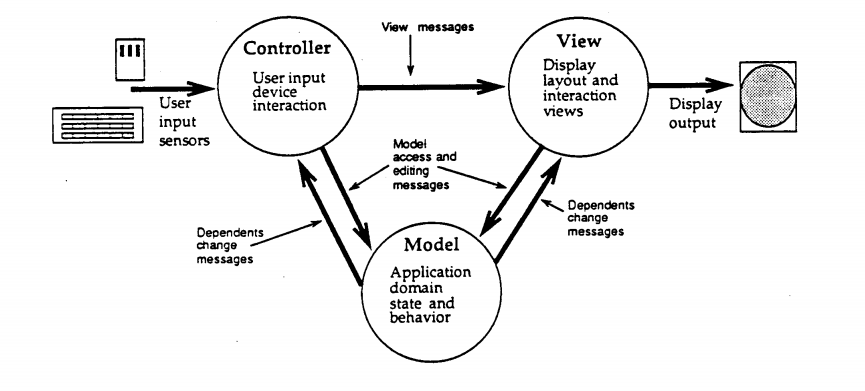
\includegraphics[width=\textwidth]{img/mvc}
	\caption[Esquema MVC]{Esquema del patrón arquitectónico Modelo-Vista-Controlador}
	\label{fig:mvc}
\end{figure}


El framework escogido para el desarrollo de twinX, Yii2, impulsa este patrón mediante su funcionamiento separado en modelos, vistas y controladores, como ya veremos en el capítulo próximo. Sin embargo, el MVC no constituye la arquitectura de la aplicación al completo, sino que también intervienen la capa de conexión con la base de datos y la capa lógica. Ambas están suministradas por el propio framework, con el manejo de las mismas de forma interna, dando acceso a ellas a través de objetos.